\vspace{1em}
\scalebox{0.85}{
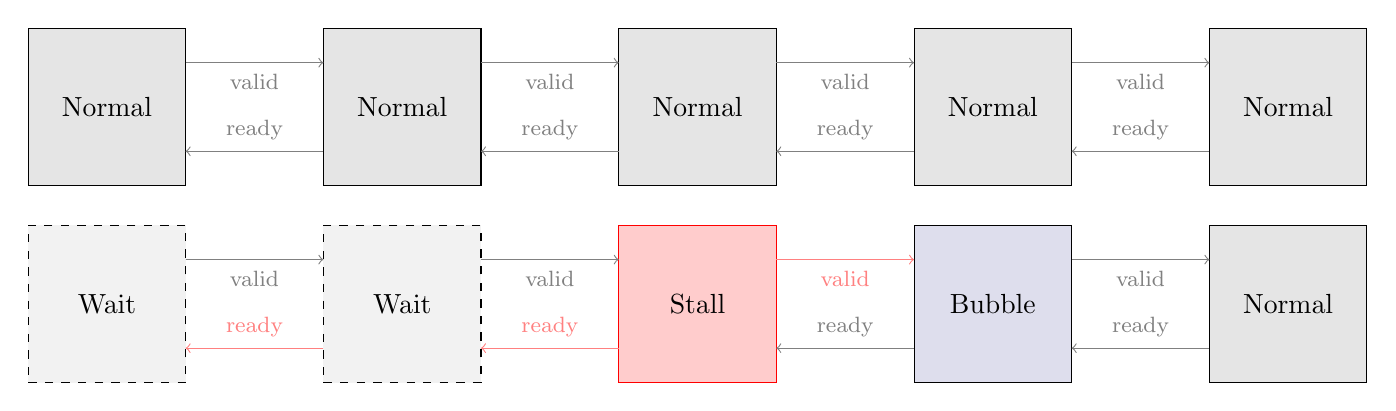
\begin{tikzpicture}[scale=1.25, draw=gray, inner sep=0, outer sep=0]
% STEP 1
  \node[rectangle, draw=black,
    align=center,
    minimum height = 2cm,
    minimum width = 2cm,
    fill = gray!20] (stage3_1) at (0, 0) {Normal};
  \node[rectangle, draw=black,
    align=center,
    minimum height = 2cm,
    minimum width = 2cm,
    fill = gray!20] (stage2_1) at (-3, 0) {Normal};
  \node[rectangle, draw=black,
    align=center,
    minimum height = 2cm,
    minimum width = 2cm,
    fill = gray!20] (stage1_1) at (-6, 0) {Normal};
  \node[rectangle, draw=black,
    align=center,
    minimum height = 2cm,
    minimum width = 2cm,
    fill = gray!20] (stage4_1) at (3, 0) {Normal};
  \node[rectangle, draw=black,
    align=center,
    minimum height = 2cm,
    minimum width = 2cm,
    fill = gray!20] (stage5_1) at (6, 0) {Normal};

  \draw[->] ([yshift=0.45cm]stage1_1.east)  -- node[text=gray, below=0.15cm]{\footnotesize{valid}} ([yshift=0.45cm]stage2_1.west);
  \draw[<-] ([yshift=-0.45cm]stage1_1.east) -- node[text=gray, above=0.15cm]{\footnotesize{ready}} ([yshift=-0.45cm]stage2_1.west);

  \draw[->] ([yshift=0.45cm]stage2_1.east) -- node[text=gray, below=0.15cm]{\footnotesize{valid}} ([yshift=0.45cm]stage3_1.west);
  \draw[<-] ([yshift=-0.45cm]stage2_1.east) -- node[text=gray, above=0.15cm]{\footnotesize{ready}} ([yshift=-0.45cm]stage3_1.west);

  \draw[->] ([yshift=0.45cm]stage3_1.east) -- node[text=gray, below=0.15cm]{\footnotesize{valid}} ([yshift=0.45cm]stage4_1.west);
  \draw[<-] ([yshift=-0.45cm]stage3_1.east) -- node[text=gray, above=0.15cm]{\footnotesize{ready}} ([yshift=-0.45cm]stage4_1.west);

  \draw[->] ([yshift=0.45cm]stage4_1.east) -- node[text=gray, below=0.15cm]{\footnotesize{valid}} ([yshift=0.45cm]stage5_1.west);
  \draw[<-] ([yshift=-0.45cm]stage4_1.east) -- node[text=gray, above=0.15cm]{\footnotesize{ready}} ([yshift=-0.45cm]stage5_1.west);

% STEP 2
  \node[rectangle, draw=red,
    align=center,
    minimum height = 2cm,
    minimum width = 2cm,
    fill = red!20] (stage3_2) at (0, -2) {Stall};
  \node[dashed, rectangle, draw=black,
    align=center,
    minimum height = 2cm,
    minimum width = 2cm,
    fill = gray!10] (stage2_2) at (-3, -2) {Wait};
  \node[dashed, rectangle, draw=black,
    align=center,
    minimum height = 2cm,
    minimum width = 2cm,
    fill = gray!10] (stage1_2) at (-6, -2) {Wait};
  \node[rectangle, draw=black,
    align=center,
    minimum height = 2cm,
    minimum width = 2cm,
    fill = blue!30!gray!20] (stage4_2) at (3, -2) {Bubble};
  \node[rectangle, draw=black,
    align=center,
    minimum height = 2cm,
    minimum width = 2cm,
    fill = gray!20] (stage5_2) at (6, -2) {Normal};

  \draw[->] ([yshift=0.45cm]stage1_2.east)  -- node[text=gray, below=0.15cm]{\footnotesize{valid}} ([yshift=0.45cm]stage2_2.west);
  \draw[<-, red!50] ([yshift=-0.45cm]stage1_2.east) -- node[text=red!50, above=0.15cm]{\footnotesize{ready}} ([yshift=-0.45cm]stage2_2.west);

      \draw[->] ([yshift=0.45cm]stage2_2.east) -- node[text=gray, below=0.15cm]{\footnotesize{valid}} ([yshift=0.45cm]stage3_2.west);
  \draw[<-, red!50] ([yshift=-0.45cm]stage2_2.east) -- node[text=red!50, above=0.15cm]{\footnotesize{ready}} ([yshift=-0.45cm]stage3_2.west);

  \draw[->, red!50] ([yshift=0.45cm]stage3_2.east) -- node[text=red!50, below=0.15cm]{\footnotesize{valid}} ([yshift=0.45cm]stage4_2.west);
  \draw[<-] ([yshift=-0.45cm]stage3_2.east) -- node[text=gray, above=0.15cm]{\footnotesize{ready}} ([yshift=-0.45cm]stage4_2.west);

  \draw[->] ([yshift=0.45cm]stage4_2.east) -- node[text=gray, below=0.15cm]{\footnotesize{valid}} ([yshift=0.45cm]stage5_2.west);
  \draw[<-] ([yshift=-0.45cm]stage4_2.east) -- node[text=gray, above=0.15cm]{\footnotesize{ready}} ([yshift=-0.45cm]stage5_2.west);
\end{tikzpicture}
}
